\begin{figure*}[t]
\vspace{-2em}
\centering
\begin{subfigure}[b]{0.5\textwidth}
  \centering
  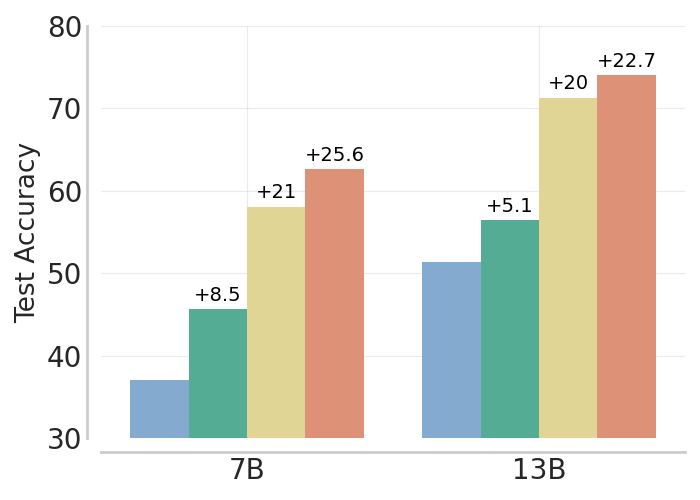
\includegraphics[scale=0.39]{icml2023/figs/abs_with_rel/gsm8k_abs_with_rel.png}
  \caption{GSM8K for 7B and 13B sizes}
    \label{fig:gsm8k}
\end{subfigure}%
\begin{subfigure}[b]{0.5\textwidth}
  \centering
  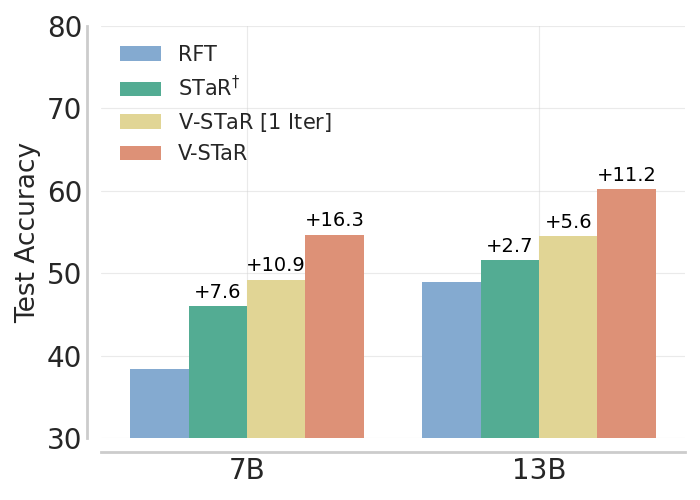
\includegraphics[scale=0.39]{icml2023/figs/abs_with_rel/mbpp_abs_with_rel.png}
  \caption{MBPP for 7B and 13B sizes}
    \label{fig:mbpp}
\end{subfigure}%
\caption{\textbf{Pass$@1$ and Best-of-64 scores for generator-only and verifier-based methods}. Numbers above each bar represent the absolute improvement over RFT. \vstar{}[1 Iter] baseline is trained with data consisting of $3\times16$ completions per query for one iteration only. \stardag and \vstar{} are trained using iterative data collection (i.e. 16 completions generated per query at each iteration). At test time, \revision{Best-of-64 is calculated using \autoref{eq:ver_at_k} on 128 candidate answers sampled per problem from the generators}. \vstar{} 7B performs on par with CodeLLaMA 34B, which has a zero-shot Pass$@1$ of 55\% on MBPP. }
\label{fig:results_rft_1iter}
\vskip -0.03in
\end{figure*}


% \vskip -0.2in